
%(BEGIN_QUESTION)
% Copyright 2006, Tony R. Kuphaldt, released under the Creative Commons Attribution License (v 1.0)
% This means you may do almost anything with this work of mine, so long as you give me proper credit

It has been known for a long time that ions (electrically charged atoms or molecules) exist in most flames.  This means a flame can act as a weak conductor of electricity.  Given a large enough voltage, we can push a measurable current through the flame:

$$\includegraphics[width=15.5cm]{i00656x01.eps}$$

Not all fuels generate the same amount of ions when burned.  Hydrogen, for instance, burns very clean and generates negligible ionic activity.  Carbon, on the other hand, easily ionizes in flame, and so hydrocarbon fuels such as methane (CH$_{4}$), ethane (C$_{2}$H$_{6}$), and propane (C$_{3}$H$_{8}$) generate ions in approximate proportion to their carbon content.

\vskip 10pt

Explain how the circuit shown above functions, and how it would respond to the combustion of different fuel types.

\vskip 10pt

Explain how this circuit would respond if the ``fuel gas'' happened to be the discharge of a chromatograph column using hydrogen gas as the ``carrier,'' and the chromatograph were sampling a mixed-hydrocarbon stream.

\underbar{file i00656}
%(END_QUESTION)





%(BEGIN_ANSWER)

Fuel gases with greater carbon content will generate greater voltage readings on the AC meter.

%(END_ANSWER)





%(BEGIN_NOTES)

Sensing the output of a chromatograph column, this detector (FID) will produce intermittent readings corresponding to the arrival of different hydrocarbon species at the detector, separated from one another by the retarding action of the stationary phase in the column.





\vskip 20pt \vbox{\hrule \hbox{\strut \vrule{} {\bf Virtual Troubleshooting} \vrule} \hrule}

This question is a good candidate for a ``Virtual Troubleshooting'' exercise.  Presenting the diagram to students, you first imagine in your own mind a particular fault in the system.  Then, you present one or more symptoms of that fault (something noticeable by an operator or other user of the system).  Students then propose various diagnostic tests to perform on this system to identify the nature and location of the fault, as though they were technicians trying to troubleshoot the problem.  Your job is to tell them what the result(s) would be for each of the proposed diagnostic tests, documenting those results where all the students can see.

During and after the exercise, it is good to ask students follow-up questions such as:

\begin{itemize}
\item{} What does the result of the last diagnostic test tell you about the fault?
\item{} Suppose the results of the last diagnostic test were different.  What then would that result tell you about the fault?
\item{} Is the last diagnostic test the best one we could do?
\item{} What would be the ideal order of tests, to diagnose the problem in as few steps as possible?
\end{itemize}

%INDEX% Chemistry, ionization: in a flame
%INDEX% Measurement, analytical: carbon (in a gas)

%(END_NOTES)


